\documentclass[tikz]{standalone}

% Last Change: 19th March 2016, Original Implementation done by Sharru Moeller.
% Feel free to change, distribute and use this file any way you like.

\usepackage[english]{babel}
\usepackage{xcolor}
\usepackage[utf8]{inputenc}
\usepackage{ifthen}
\usepackage{pgfmath}
\usepackage{tikz}
\usetikzlibrary{positioning}
\usepackage{amsmath}
\usepackage{xparse}
\usepackage{etoolbox}

\newcounter{listtotal}\newcounter{listcntr}%
\NewDocumentCommand{\descs}{o}{%
  \setcounter{listtotal}{0}\setcounter{listcntr}{-1}%
  \renewcommand*{\do}[1]{\stepcounter{listtotal}}%
  \expandafter\docsvlist\expandafter{\descsArray}%
  \IfNoValueTF{#1}
    {\namesarray}% \names
    {% \names[<index>]
     \renewcommand*{\do}[1]{\stepcounter{listcntr}\ifnum\value{listcntr}=#1\relax##1\fi}%
     \expandafter\docsvlist\expandafter{\descsArray}}
}

\begin{document}

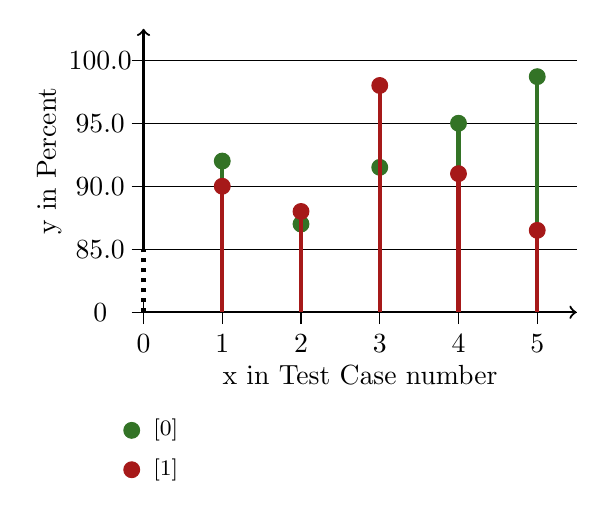
\begin{tikzpicture}

% =======================================================================================================
% Fill in your data and general axis/legend information in this section in order to generate the diagram you need
% =======================================================================================================

\def\Xscale{1}				% X-Axis Scaling
\def\Yscale{5}				% Y-Axis Scaling
\def\ySkip{16}				% how many y scaling points are to be jumped. In this case the y axis starts at 16*\Yscale, so 80. (Since this is percentage based, 80%)
\def\nDP{5} 				% Number of Data Points (x-axis length)
\def\nSP{20} 				% Number of Scaling Points (Y axis length)
\def\xDBP{1}				% Distance/Spacing between Data Point on X-Axis.
\def\yDBP{0.8}				% Distance/Spacing between Data Point on Y-Axis.
\def\Data{{{92, 87, 91.5, 95, 98.7},{90, 88, 98, 91, 86.5}}}		% Array of Array of Data. Every array introduces a new color in the Diagram
\def\nMDL{2}				% The number of multiple Data Arrays to do in one tikzpic
\def\colorIn{{"0.2 0.45 0.15","0.65 0.10 0.10","0.10 0.20 0.65","0.00 0.00 0.52","0.00 0.00 0.00","0.00 0.00 0.00"}}	% Array of Colors. Will be used in succession
\newcommand{\descsArray}{Anomaly Detection Rate, Pattern Detection Rate, Desc C, Desc D, Desc D, Desc E}				% Array of Color Descriptions. Will be filled in to the legend
%\def\title{Pattern- and Anomaly Detection}
\def\yAxis{y in Percent}				% X-Axis Description
\def\xAxis{x in Test Case number}		% Y-Axis Description

% =======================================================================================================
% This part changes spacings of all sorts. Feel free to change, but this is a useful base setup
% =======================================================================================================

\def\ydTD{0.55}			% x Distance of Data Lines to their Descriptor
\def\xdTD{0.4}			% y Distance of Data Lines to their Descriptor
\def\dSLL{0.15}			% Length of Data Lines Points
\def\cSize{0.1}			% Circle Size
\def\nMDLDist{0.1}		% for bottom up line Diagrams, distance between lines
\def\titleDist{1}		% Distance to title
\def\xDescDist{0.8}		% Distance of x axis description
\def\yDescDist{1.2}		% Distance of y axis description
\def\rleft{1}			% frame left. The frame values add possibilities of adding whitespae around the figure.
\def\rdown{0}			% frame down
\def\rright{0}			% frame right
\def\rup{0}				% frame up
\def\legendDist{1.6}		% Distance to Legend below (between xAxis and legend)
\def\legendSpac{0.5}		% Spacing between legend parts
\def\legendRightIndent{-0.2}	% Indent to Legend

% =======================================================================================================
% This part is the actual file. It isn't very well documented currently. It was originally made on a whim. Will be updated once I find the time/need to.
% =======================================================================================================

%\node at (\nDP*\xDBP/2+1-\xDBP*0.5/2,\titleDist+\yDBP*\nSP-\ySkip*\yDBP) {\Large \title};
\node at (\nDP*\xDBP/2+0.5-\xDBP*0.5/2,-1*\xDescDist) {\xAxis};
\node [rotate=90] at (-1*\yDescDist,  {(\nSP-\ySkip+\yDBP)*\yDBP/2}) {\yAxis};

% Coordinate System Line
\ifthenelse{\ySkip>0}{
	\draw[dotted, ultra thick] (0,0)--(0,\yDBP);
	\draw[->, thick] (0, \yDBP)--(0, \nSP*\yDBP+\yDBP*0.5-\ySkip*\yDBP);
	\draw[->, thick] (0, 0)--(\nDP*\xDBP+1-\xDBP*0.5, 0);
} {
	\draw[<->, thick] (0, \nSP*\yDBP+\yDBP*0.5)|-(\nDP*\xDBP+1-\xDBP*0.5, 0);
}

% Data Position Lines with Scaling (aka initialize x and y axis)
\foreach \i in {0,...,\nDP}
{
	\draw (\i*\xDBP, -1*\dSLL) -- (\i*\xDBP, \dSLL);
	\pgfmathparse{\i*\Xscale};
	\node at(\i*\xDBP, -1*\xdTD) {\pgfmathparse{int(\i*\Xscale)}\pgfmathresult};
}
\pgfmathparse{\nSP-1}
\foreach \i in {\ySkip,...,\pgfmathresult}
{
	\draw (-1*\dSLL, \i*\yDBP-\ySkip*\yDBP+\yDBP) -- (\nDP*\xDBP+1-\xDBP*0.5, \i*\yDBP-\ySkip*\yDBP+\yDBP);
	\node at(-1*\ydTD, \i*\yDBP-\ySkip*\yDBP+\yDBP) {\pgfmathparse{(\i+1)*\Yscale}\pgfmathresult};
}
\draw (-1*\dSLL, 0) -- (\nDP*\xDBP+1-\xDBP*0.5, 0);
\node at(-1*\ydTD, 0) {0};

% Data Lines (aka visualize the data)
\pgfmathparse{\nMDL-1}
\foreach \k in {0,...,\pgfmathresult}
{
	\pgfmathparse{\colorIn[\k]}
	\definecolor{currentColor}{rgb}{\pgfmathresult}
	% Bottom Up Single Line (linediagram v1)
	\pgfmathparse{\nDP-1};
	\foreach \i in {0,...,\pgfmathresult}
	{
		\draw[ultra thick, currentColor] (\i*\xDBP+\xDBP, 0)--(\i*\xDBP+\xDBP, \yDBP*\Data[\k][\i]/\Yscale-\ySkip*\yDBP);
		\draw[fill, currentColor] (\i*\xDBP+\xDBP, \yDBP*\Data[\k][\i]/\Yscale-\ySkip*\yDBP) circle (\cSize);
	}
}

%Legend
\pgfmathparse{\nMDL-1}
\foreach \k in {0,...,\pgfmathresult}
{
		\pgfmathparse{\colorIn[\k]}
		\definecolor{currentColor}{rgb}{\pgfmathresult};
		% \draw[currentColor, fill=currentColor] (\legendRightIndent, -1*\legendDist-\legendSpac*\k) rectangle (\legendRightIndent+0.2, -1*\legendDist-\legendSpac*\k+0.2);
		\draw[currentColor, fill=currentColor] (\legendRightIndent+\cSize/2, -1*\legendDist-\legendSpac*\k+\cSize) circle (\cSize);
		\node[anchor=west] at (\legendRightIndent+0.2, -1*\legendDist-\legendSpac*\k+0.1) {\footnotesize \descs[\k]};
}

\draw[opacity=0] (-1*\rleft, -1*\rdown)--(\nDP*\xDBP+1-\xDBP*0.5+\rright, -1*\rdown)--(\nDP*\xDBP+1-\xDBP*0.5+\rright, \nSP*\yDBP+\yDBP*0.5-\ySkip*\yDBP+\rup)--(-1*\rleft,\nSP*\yDBP+\yDBP*0.5-\ySkip*\yDBP+\rup);



\end{tikzpicture}

\end{document}

